%*****************************************
\chapter{Metrología óptica}\label{ch:metrologiaoptica}
%*****************************************

En este capítulo se brinda una mirada general de la metrología óptica.
En la primer sección se realiza una introducción a los sistemas ópticos de medición, sus ventajas y desventajas y se realiza una clasificación general en base a su principio de funcionamiento.
En la segunda sección se trata en detalle el principio de triangulacíon, la base de los sensores más conocidos y utilizados.
En las secciones a continuación se explican los principales métodos de medición basados en triangulación: en la tercer sección se explican los sensores basados en visión estéreo, en la cuarta sección se describen los sensores conocidos como escaneres de línea, y finalmente en la quinta sección se explicará en detalle el funcionamiento de las distintas variantes de los métodos conocidos como luz estructurada, una de las cuales será utilizada para el desarrollo de este proyecto.

\section{Introducción}
En la \autoref{fig:canonicalOpticalSensor} se observa el esquema de un sensor 3D óptico genérico. Básicamente se observa una fuente de luz, el objeto y el sensor que observa la interacción entre el objeto y la luz. La iluminación puede ser implementada de diversas formas y suele tener un efecto importante en la performance del sensor. Por ejemplo, la iluminación puede ser coherente o incoherente, directa o difusa, estructurada o homogénea, monocromatica o multicromatica, polarizada o no, y temporalmente continua o pulsada.

\begin{figure}[bth]
    \myfloatalign
        {\includegraphics[width=0.9\linewidth]{images/genericOptical3DSensor}}
        \caption{Esquema genérico de un sensor 3D óptico}
        \label{fig:canonicalOpticalSensor}
\end{figure}

La luz incide sobre el objeto observado e interactúa con los átomos que lo conforman. Generalmente se produce scattering coherente, por lo que la luz reflejada está en fase con la luz proveniente de la fuente. El scattering coherente genera una limitación fundamental, conocida como ruido speckle, que será explicado más adelante. Para evitarlo se puede utilizar una excitación térmica o se pueden aprovechar los efectos de la fluorescencia, pero ambos temas exceden el alcance de este trabajo y no serán tratados.

Por otro lado, la interacción de la luz con la superficie puede causar reflexión difusa o especular (como un espejo), y se puede producir en la superficie o dentro del volumen del objeto (como se produce por ejemplo en la piel humana, o en plásticos).

La luz reflejada (o generada) por el objeto contiene mucha información, principalmente intensidad y color (como en fotografía), amplitud compleja (como en interferometría y holografía), polarización, coherencia y tiempo de vuelo. Estas características pueden ser combinadas y utilizadas para obtener la forma 3D de la superficie.

Los sistemas ópticos de medición ofrecen varias ventajas respecto a los tradicionales métodos de medición por contacto, sobre todo en ambientes y procesos industriales. Las que más nos interesan son su velocidad y el hecho de que no entran en contacto con la pieza, lo que permite por ejemplo realizar mediciones sin comprometer la integridad del propio dispositivo de medición.

Los sensores ópticos pueden clasificarse en cuatro grandes categorías a partir de las características de la incerteza en su medición \cite{hausler2011limitations}:
\begin{enumerate}
    \item Triangulación
    \item Interferometría de escaneado coherente y tiempo de vuelo
    \item Interferometría clásica
    \item Deflectometría
\end{enumerate}

El tipo 1 incluye todos los sensores basados en triangulación: triangulación laser, luz estructurada, visión estereo, microscopía confocal, \emph{shape from focus}, \emph{shape from defocus}, etc. Los sensores de triangulación generalmente miden a partir de la deformación lateral provocada por la perspectiva. La incerteza de la medición queda determinada principalmente por la incerteza de la medición de este desplazamiento. A partir de un simple análisis geométrico se puede observar que la incerteza de la medición escala cuadráticamente con la distancia, como se explica en \cite{khoshelham2012accuracy}. En el caso de la medición de objetos rugosos la fuente de ruido dominante es el producido por los speckles, de los cuales hablaremos más adelante. Vamos a denominar a este tipo de sensores como sensores del tipo 1a. Para superficies suaves o para triangulación con fluorescencia, la fuente de ruido dominante es el ruido fotónico (ver \autoref{ch:noiseSourcesDigitalCamera}). Denominaremos a este tipo de sensores como tipo 1b.

En la \autoref{fig:triangulationLaserSensor} se muestra una representación de un sensor de triangulación. En este caso se trata de un sensor del tipo 1a, con una fuente de luz laser puntual. El haz de luz se enfoca sobre un eje de proyección hacia la superficie de un objeto rugoso. El punto es observado mediante un sistema óptico, sobre el eje de observación. El eje de proyección y el eje de observación determinan el ángulo de triangulación $\theta$. A partir de la ubicación del punto sobre la imagen y de la geometría del sensor se puede calcular la distancia $z$. 
En la parte derecha de la figura se puede observar un ejemplo de cómo se ve el punto laser en la imagen obtenida por la cámara. Se nota que se produce interferencia constructiva y destructiva (debido a la rugosidad del objeto sumado al uso de una fuente de luz laser, es decir, luz coherente). Este efecto hace difícil determinar con precisión la ubicación exacta del punto, y es la fuente de ruido que mencionamos previamente, conocido como ruido speckle\footnote{\url{http://en.wikipedia.org/wiki/Speckle_noise}}.

%        {\includegraphics[width=1.0\linewidth]{images/triangulationLaserSensor}}
%\begin{figure}[bth]
%    \myfloatalign
%        {\includegraphics[width=1.0\linewidth]{images/genericLaserTriangulationSensor}}
%        \caption{Triangulación láser}
%        \label{fig:triangulationLaserSensor}
%\end{figure}

\begin{figure}[bth]
    \myfloatalign
        \myfloatalign
        \subfloat[Esquema del sensor]
        {\includegraphics[width=0.69\linewidth]{images/genericLaserTriangulationSensor}}
%	\quad
        \subfloat[Efecto speckle]
        {\includegraphics[width=.29\linewidth]{images/laserPointSpeckle}}
        \caption{Triangulación láser}
        \label{fig:triangulationLaserSensor}
\end{figure}

Los sensores del tipo 2 incluyen los sensores de tiempo de vuelo y los denominados \ac{CSI} en superficies rugosas (también conocidos como radar de coherencia). 
En la \autoref{fig:whiteLightInterferometer} se puede observar el esquema de uno de ellos. Cada haz de luz proveniente de la fuente de luz pasa por una lente colimadora, luego el beam splitter lo divide en $2$, de los cuales uno viaja hacia el objeto y el otro hacia un espejo de referencia. El reflejo de ambos vuelve al dispositivo, pasa nuevamente por el beam splitter, luego por otra lente y finalmente llegan al mismo punto del sensor de la cámara. Si la distancia recorrida por cada uno es exactamente igual, se producirá interferencia constructiva, y en caso contrario se produce interferencia destructiva. De esta forma, para cada ubicación del espejo de referencia se obtiene un valor para cada pixel. Evaluando esta funcion temporal de cada pixel se puede obtener con gran precisión el valor $z$ correspondiente.
Para superficies rugosas la principal fuente de ruido es la micro-topografía de la superficie misma. Un aspecto muy interesante de este tipo de sensores es que la incerteza de la medición no escala con la distancia o con la apertura de observación. Esto permite medir agujeros profundos o realizar mediciones a larga distancia sin incrementar la incerteza de la medición. Sin embargo el método no es muy eficiente ya que requiere tomar una gran cantidad de imágenes variando la posición del espejo de referencia. 

\begin{figure}[bth]
    \myfloatalign
        {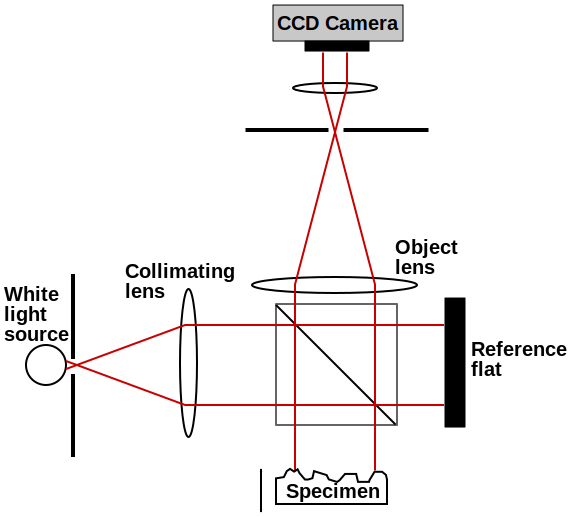
\includegraphics[width=0.8\linewidth]{images/whiteLightInterferometer}}
        \caption{Interferómetro de luz blanca}
        \label{fig:whiteLightInterferometer}
\end{figure}

Los sensores del tipo 3 son los interferómetros clásicos para medir superficies suaves y especulares. La mayor fuente de ruido es el ruido fotónico. La interferometría clásica puede obtener una incerteza de medición de niveles sub-nanómetro, en ambientes adecuados. Los interferómetros clásicos, a diferencia del radar de coherencia, realizan un promediado lateral de la topografía.

Por último, los sensores del tipo 4 incluyen deflectometría y deflectometría de micro-escala. Los sensores del tipo 4 realizan una medición implícita a partir de la variación de la forma de la superficie en vez de medir la altura directamente. La derivada espacial se genera ópticamente, por lo que la topografía obtenida mediante integración numérica puede obtener un nivel de ruido muy bajo, del orden de los nanómetros. En la \autoref{fig:deflectometrySensor} se puede observar un esquema de un sensor de este tipo.

\begin{figure}[bth]
    \myfloatalign
        {\includegraphics[width=0.85\linewidth]{images/deflectometrySensor}}
        \caption{Principio de funcionamiento de un sensor de deflectometría}
        \label{fig:deflectometrySensor}
\end{figure}

En la \autoref{tab:sensorTypeComparison} se muestra una comparación de los distintos tipos de sensores para diversos tipos de superficie. Como se puede observar no existe el sensor ideal, y es de suma importancia la elección del tipo de sensor adecuado para cada situación particular.

\begin{table}[!bth] 
    \myfloatalign
    \begin{tabularx}{\textwidth}{ l X | c | c | c | c | c }
    & & \multicolumn{5}{c}{Tipo de sensor} \\[2ex]
    & & \rotatebox{90}{\shortstack[l]{Triangulación\\laser (tipo 1a)}} & \rotatebox{90}{\shortstack[l]{Luz estructurada\\(tipo 1a)}} & \rotatebox{90}{\shortstack[l]{CSI\\(tipo 2)}} & \rotatebox{90}{\shortstack[l]{Interferometría\\clásica (tipo 3)}} & \rotatebox{90}{\shortstack[l]{Deflectometría\\(tipo 4)}} \\ \hline
    & Especular, plana & - - & - - & ++ & ++ & ++ \\ 
    & Especular, curva & - - & - - & $0$ & $0$ & ++ \\ 
    & Mate / Lambertiana & + & ++ & ++ & - - & - - \\ 
    & Maquinada & $0$ & $0$ & ++ & - - & - \\ 
    & Maquinada, inclinada & - & $0$ & + & - - & - \\ 
    & Agujeros profundos & - - & - - & + & - - & - - \\ 
    \rotatebox{90}{\rlap{~~~Tipo de superficie}} & Piel / plástico & - & $0$ & + & - - & - - \\
    \hline
    \multicolumn{7}{c}{\small- - inaplicable; - no recomendable; $0$ neutro; + aplicable; ++ específico} \\
    \end{tabularx}
    \caption{Comparación de los distintos tipos de sensores ópticos}
    \label{tab:sensorTypeComparison}
\end{table}

\section{Principio de triangulación}
El principio de triangulación se basa en la premisa de que la luz se mueve en línea recta (en medios homogéneos), lo que permite derivar las ecuaciones de reconstrucción 3D a partir de conceptos básicos de geometría tridimensional como intersecciones entre líneas y planos, o intersecciones aproximadas entre pares de líneas\footnote{En tres dimensiones dos líneas pueden no intersectarse, aún cuando no son paralelas. El punto de intersección se reemplaza por el punto que minimiza las distancias a las rectas}.

Las técnicas basadas en triangulación más utilizadas son visión estéreo, escáner de línea y luz estructurada. Las tres se basan en el mismo principio de triangulación pero funcionan de manera diferente, y cada una tiene sus ventajas y desventajas. Más adelante se analizará en detalle cada una de ellas, pero antes de avanzar veremos una breve introducción a los principios matemáticos involucrados.

\subsection{Intersección línea-plano}
El cálculo de la intersección entre una línea y un plano es sencillo cuando usamos la representación parámetrica de la línea \cite{lanman2009build}
    \[ L = \{ p=q_L + \lambda v : \lambda \in \mathbb{R}  \} \]
y la representación implícita del plano
    \[ P = \{ p : n^T (p - q_P) = 0 \} \]
con $q_L$ un punto perteneciente a la línea y $v$ su vector dirección, siendo $n$ el vector normal al plano y $q_P$ un punto perteneciente a éste.

\begin{figure}[bth]
    \myfloatalign
        {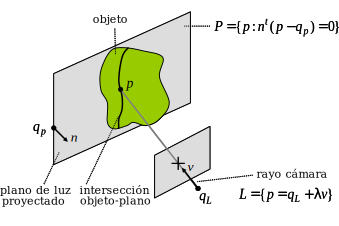
\includegraphics[width=0.85\linewidth]{images/intersectionPlaneLine}}
        \caption{Intersección línea-plano}
        \label{fig:intersecionPlaneLine}
\end{figure}

Como se puede notar, puede que la línea y el plano no se intersecten, en cuyo caso decimos que la línea y el plano son paralelos. Este caso sucede cuando el vector dirección de la línea $v$ y el vector normal al plano $n$ son ortogonales ($n^T v = 0$). También puede suceder que la línea esté contenida en el plano. Si los vectores $v$ y $n$ no son ortogonales, entonces la línea y el plano intersectan en un sólo punto $p$. Como este punto pertenece a la línea, podemos escribirlo como $p = q_L + \lambda v$, donde $\lambda$ es el valor que debemos determinar. Como el punto también pertenece al plano, $\lambda$ debe satisfacer también la ecuación
    \[ n^T (p - q_P) = n^T (\lambda v + q_L - q_P) = 0 \]
o de manera equivalente
    \begin{equation*}
        \lambda = \frac {n^T (q_P - q_L)} {n^T v}
    \end{equation*}

%Como asumimos que la línea y el plano no eran paralelos (para lo cual chequeamos previamente que $n^T v \neq 0$), esta expresión está bien definida.

\subsection{Intersección línea-línea}
Ahora vamos a considerar la intersección entre dos líneas arbitrarias $L_1$ y $L_2$
    \[ L_1 = \{ p=q_1 + \lambda_1 v_1 : \lambda_1 \in \mathbb{R}  \} \]
y
    \[ L_2 = \{ p=q_2 + \lambda_2 v_2 : \lambda_2 \in \mathbb{R}  \} \]

\begin{figure}[bth]
    \myfloatalign
        {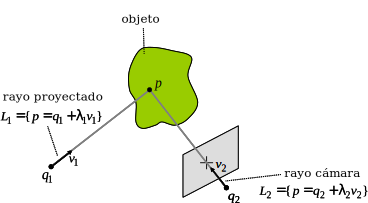
\includegraphics[width=0.9\linewidth]{images/intersectionLineLine}}
        \caption{Intersección línea-línea}
        \label{fig:intersecionLineLine}
\end{figure}

Primero analizaremos los casos especiales. Los vectores $v_1$ y $v_2$ pueden ser linealmente dependientes (es decir uno es un múltiplo escalar del otro) o independientes. 
Las dos líneas son paralelas si los vectores $v_1$ y $v_2$ son linealmente dependientes. Si además el vector $q_2 - q_1$ también es un múltiplo de $v_1$ o $v_2$, entonces las líneas son idénticas. Por otro lado, en el caso que las líneas son paralelas pero no identicas, las líneas no se intersectan.
Si $v_1$ y $v_2$ son linealmente independientes, las líneas pueden intersectar o no. Si las líneas intersectan, la intersección contiene un sólo punto. En este caso, las condiciones necesarias y suficientes para que dos líneas se intersecten es que los valores escalares $\lambda_1$ y $\lambda_2$ existan tal que
    \[ q_1 + \lambda_1 v_1 = q_2 + \lambda_2 v_2 \]
o de manera equivalente que el vector $q_2 - q_1$ sea linealmente dependiente de $v_1$ y $v_2$.

Como dos líneas pueden no intersectar (lo que sucede muchas veces), vamos a definir la intersección aproximada como el punto que esté más cerca de las dos líneas. Para ser más precisos, vamos a definir la intersección aproximada como el punto $p$ que minimiza la suma del cuadrado de las distancias a ambas líneas, sin importar si las líneas intersectan o no
    \[ \phi(p, \lambda_1, \lambda_2) = \| q_1 + \lambda_1 v_1 - p \|^2 + \| q_2 + \lambda_2 v_2 - p \|^2  \]
    
Al igual que anteriormente, asumimos que $v_1$ y $v_2$ son linealmente independientes de manera tal que la intersección es un punto único.

Para determinar el valor de $p$ vamos a utilizar un enfoque algebraico. La funcion $\phi(p, \lambda_1, \lambda_2)$ es una función cuadrática y no-negativa de cinco variables, las tres coordenadas del punto $p$ y los dos escalares $\lambda_1$ y $\lambda_2$.

Primero procedemos a reducir el problema a la minimización de una función cuadrática no-negativa de sólo dos variables $\lambda_1$ y $\lambda_2$. 
Para ello comenzaremos definiendo los puntos $p_1 = q_1 + \lambda_1 v_1$ y $p_2 = q_2 + \lambda_2 v_2$, y el punto $p_{12}$ como el punto medio entre ellos:
    \[ p_{12} = p_1 + \frac{1}{2} (p_2 - p_1) = p_2 + \frac{1}{2} (p_1 - p_2) \]

Una condición necesaria para el mínimo $(p, \lambda_1, \lambda_2)$ de $\phi$ es que las derivadas parciales de $\phi$ respecto a las cinco variables, todas se hagan cero en el mínimo. En particular, las tres derivadas respecto a las coordenadas del punto $p$ deben cumplir:
    \[ \frac{\partial \phi}{\partial p} = (p - p_1) + (p - p_2) = 0 \]
Por lo tanto es necesario que el punto mínimo $p$ sea el punto medio $p_{12}$ del segmento que une $p_1$ con $p_2$.

Con este resultado el problema se reduce a la minimización del cuadrado de la distancia de un punto $p_1$ en la línea $L_1$ hacia un punto $p_2$ en la línea $L_2$, es decir, sólo debemos minimizar la función cuadrática no-negativa de dos variables:
    \[ \psi  (\lambda_1, \lambda_2) = 2 \phi(p_{12}, \lambda_1, \lambda_2) = \| (q_2 + \lambda_2 v_2) - (q_1 + \lambda_1 v_1) \| ^2 \]
    
Como se mencionó previamente, también es necesario que las dos derivadas parciales de $\psi$ respecto a $\lambda_1$ y $\lambda_2$ sean iguales a cero en el mínimo:
    \[ \frac{\partial \psi}{\partial \lambda_1} = v_1^T (\lambda_1 v_1 - \lambda_2 v_2 + q_1 - q_2) = \lambda_1 \| v_1 \|^2 - \lambda_2 v_1^T v_2 + v_1^T (q_1 - q_2) = 0 \]
    \[ \frac{\partial \psi}{\partial \lambda_2} = v_2^T (\lambda_2 v_2 - \lambda_1 v_1 + q_2 - q_1) = \lambda_2 \| v_2 \|^2 - \lambda_2 v_2^T v_1 + v_2^T (q_2 - q_1) = 0 \]

Estas ecuaciones lineales en $\lambda_1$ y $\lambda_2$ pueden ser expresadas en forma matricial como:
\[ 
    \begin{bmatrix}
        \|v_1\|^2  & -v_1^T v_2 \\
        -v_2^T v_1 & \|v_2\|^2
    \end{bmatrix}
    \begin{bmatrix} 
        \lambda_1 \\ 
        \lambda_2
    \end{bmatrix}
    = 
    \begin{bmatrix}
        v_1^T (q_2 - q_1) \\
        v_2^T (q_1 - q_2)
    \end{bmatrix} 
\]

Debido a la independencia lineal entre $v_1$ y $v_2$ la matriz de 2x2 de la izquierda es no-singular. De esta forma la solución única queda dada por:
\[ 
    \begin{bmatrix} 
        \lambda_1 \\ 
        \lambda_2
    \end{bmatrix}
    =
    \begin{bmatrix}
        \|v_1\|^2  & -v_1^T v_2 \\
        -v_2^T v_1 & \|v_2\|^2
    \end{bmatrix}
    ^{-1}
    \begin{bmatrix}
        v_1^T (q_2 - q_1) \\
        v_2^T (q_1 - q_2)
    \end{bmatrix}
\]
o de manera equivalente:
\[ 
    \begin{bmatrix} 
        \lambda_1 \\ 
        \lambda_2
    \end{bmatrix}
    =
    \frac{1}{ \|v_1\|^2 \|v_2\|^2 -(v_1^T v_2)^2 }
    \begin{bmatrix}
        \|v_2\|^2  & v_1^T v_2 \\
        v_2^T v_1  & \|v_1\|^2
    \end{bmatrix}
    \begin{bmatrix}
        v_1^T (q_2 - q_1) \\
        v_2^T (q_1 - q_2)
    \end{bmatrix}
\]

Finalmente la intersección aproximada puede obtenerse a partir del valor de $\lambda_1$ o $\lambda_2$.

\section{Visión estéreo}
Visión estéreo consiste en dos o más cámaras que observan el mismo objeto desde diferentes ubicaciones, y la triangulación se obtiene a partir de la identificación de los pixels en cada imágen que corresponden a un mismo punto del objeto. Esta técnica tiene la ventaja de ser rápida (sólo requiere una imagen de cada cámara) pero la dificultad en establecer las correspondencias entre las imágenes hace que su precisión no sea buena. Por otro lado su aplicación resulta sumamente limitada en el caso de objetos homogéneos ya que se torna muy dificil (en ocasiones imposible) encontrar las correspondencias. En la \autoref{fig:stereoVision} se puede observar un ejemplo para ayudar a entender el principio de funcionamiento de este tipo de sensores.

%\begin{figure}[!bth]
%    \myfloatalign
%        \subfloat[Un objeto visto desde las dos cámaras]
%        {\includegraphics[width=0.9\linewidth]{images/stereoVision}}
%        \\
%        \subfloat[Dos objetos a distinta distancia z]
%        {\includegraphics[width=0.9\linewidth]{images/stereoVision2}}
%        \caption{Visión estéreo}
%        \label{fig:stereoVision}
%\end{figure}

\begin{figure}[!bth]
    \myfloatalign
        {\includegraphics[width=0.8\linewidth]{images/stereoVision2}}
        \caption{Visión estéreo}
        \label{fig:stereoVision}
\end{figure}

\section{Escáner de línea}
Un escáner de línea consiste en un generador de una línea de luz (generalmente un láser) y una cámara que observa la incidencia de la línea de luz sobre el objeto, como se observa en la \autoref{fig:laserStripe}. La reflexión de la luz que incide sobre el objeto es captada por la cámara y, conociendo la distancia y el ángulo entre el plano de luz y la cámara, a partir de una triangulación se puede obtener el perfil del objeto en la zona iluminada. Estos sistemas permiten obtener muy buena precisión, pero se debe notar que sólo se obtiene la geometría del objeto sobre una línea. Para obtener la geometría del objeto completo (o de una zona de interés) hace falta mover una de las partes (el objeto o el escáner), lo que implica un incremento considerable en el tiempo de medición y agrega una nueva fuente de error debido al sistema de desplazamiento, entre otras cosas.

\begin{figure}[!bth]
    \myfloatalign
        {\includegraphics[width=0.9\linewidth]{images/laserStripe}}
        \caption{Escáner de línea}
        \label{fig:laserStripe}
\end{figure}

\section{Luz estructurada}
Los sistemas de luz estructurada aceleran el proceso de medición a partir de la proyección de patrones de luz estructurada sobre el objeto. Una cámara observa la distorsión de estos patrones al ser reflejados y, al igual que los métodos anteriores, mediante triangulación se obtiene información tridimensional del objeto. Su principal ventaja es la flexibilidad, ya que la precisión, resolución y velocidad dependerán en gran medida del tipo de patrones que se proyectan (entre otras cosas).

Los sistemas de luz estructurada consisten de un generador de patrones de luz y al menos una cámara. Un patrón de luz 1D (línea) o 2D (grilla) es proyectado sobre el objeto y la cámara se utiliza para determinar la deformación producida. En la \autoref{fig:digitalFringeProjection} se muestra el esquema de un sistema de luz estructurada típico.

%\begin{figure}[bth]
%    \myfloatalign
%        {\includegraphics[width=1.0\linewidth]{images/structuredLightSystemDiagram}}
%        \caption{Esquema de un sistema de luz estructurada}
%        \label{fig:structuredLightSystemDiagram}
%\end{figure}

\begin{figure}[bth]
    \myfloatalign
        {\includegraphics[width=1.0\linewidth]{images/digitalFringeProjection}}
        \caption{Sistema de luz estructurada típico}
        \label{fig:digitalFringeProjection}
\end{figure}

Los patrones de luz estructurada se diseñan de manera tal que cada pixel o linea de pixeles tenga un código único que pueda ser capturado por la cámara. Solamente se puede medir áreas iluminadas por el proyector y a la vez observadas por la cámara, por lo que si el objeto es muy grande o se quiere medir toda la vuelta se deberá mover el objeto (o el sistema de medición).

En la \autoref{fig:structuredLightSequence} se muestra la secuencia de pasos estándar de un sistema de medición basado en luz estructurada.

\begin{figure}[bth]
    \myfloatalign
        {\includegraphics[width=0.8\linewidth]{images/structuredLightSequence}}
        \caption{Secuencia de pasos un sistema de luz estructurada}
        \label{fig:structuredLightSequence}
\end{figure}

El primer paso es la calibración del sistema para obtener la posición relativa del proyector de patrones y de la/s cámara/s, y para mejorar la exactitud y precisión considerando la distorsión producida por la óptica de la/s cámara/s y, en el caso que sea necesario, del proyector.

El paso siguiente es la proyección de el/los patron/es de luz estructurada y la obtención de la imagen correspondiente a cada uno de ellos. Una vez obtenidas las imágenes, estas deben ser procesadas para obtener la información requerida. La primer tarea es decodificar los patrones, es decir obtener la correspondencia entre cada pixel de la imagen y la línea o pixel del patrón de luz estructurada. Al igual que un escáner de línea (en el caso de patrones de líneas -1D-) o un sistema de visión estéreo (para patrones 2D), a partir de las correspondencias se utiliza la triangulación para obtener información sobre los puntos en tres dimensiones. Este conjunto de puntos 3D es conocido típicamente como nube de puntos. La nube de puntos no contiene información sobre la conexión entre pares de puntos, por lo que en ciertos casos se debe utilizar otro método para reconstruir la superficie a partir de la nube de puntos.

\subsection{Patrones de luz estructurada}
A través de los años se desarrollaron diversos tipos de patrones de luz estructurada. La elección del tipo apropiado depende de los requerimientos de resolución espacial, de las características del objeto a medir, de la robustez de la decodificación, de la velocidad, etc. A continuación se brinda un pequeño resumen de los más utilizados.

\subsubsection{Patrones 2D}
El caso más conocido de la utilización de patrones de luz estructurada 2D es el sensor 3D Microsoft Kinect\footnote{\url{http://en.wikipedia.org/wiki/Kinect}}, desarrollado originalmente para la consola de videojuegos XBOX 360\footnote{\url{http://en.wikipedia.org/wiki/Xbox_360}}. Este sistema utiliza luz infrarroja para proyectar un patrón de puntos sobre la escena, los cuales son observados por una cámara ubicada a un costado. Los puntos establecen una codificación 2D. La calibración del sistema permite obtener la correspondencia entre un grupo de puntos y una zona de la imagen. Este tipo de patrones permite obtener la información requerida para la triangulación a partir de una sola imagen, como es el caso de visión estéreo, pero el uso del patrón de luz estructurada facilita y hace más robusta la detección de correspondencias. Esto permite lograr altas velocidades y observar escenas dinámicas (como es el caso requerido para el control de una consola de videojuegos), pero tienen como desventaja una pobre resolución espacial/lateral.

\begin{figure}[bth]
    \myfloatalign
        {\includegraphics[width=1.0\linewidth]{images/structuredLightKinectExample}}
        \caption{Patrón infrarrojo usado por el sensor Microsoft Kinect}
        \label{fig:structuredLightKinectExample}
\end{figure}

\subsubsection{Patrones 1D binarios}
\label{sec:structuredLightBinary1DPatterns}
Los patrones binarios utilizan solamente dos valores, $0$ o $1$, los cuales son proyectados secuencialmente de manera que cada pixel es asociado a una cadena única de valores binarios. Generalmente se utilizan en líneas, tanto verticales como horizontales, de manera que $\log_2(m)$ patrones son requeridos para codificar $m$ filas (o columnas) de pixeles. La decodificación de este tipo de patrones es muy robusta debido a que cada pixel corresponde a una única fila (o columna). Sin embargo la gran cantidad de patrones requeridos imposibilita su uso en escenas dinámicas (donde el objeto está en movimiento), o bien requieren que tanto la cámara como el proyector sean capaces de trabajar a altas velocidades de adquisición/proyección.

Para generar la cadena única de valores binarios que identifican las filas (o columnas) de los patrones se utiliza generalmente un código Gray\footnote{\url{http://en.wikipedia.org/wiki/Gray_code}}. El uso de este tipo de código binario reduce las consecuencias en caso de producirse un error de decodificación. Esto se debe a que la distancia de Hamming entre códigos de Gray sucesivos es de uno. Para entender mejor supongamos un pixel que cae en el límite entre una columna y otra (ver pixel indicado con recuadro rojo en la \autoref{fig:structuredLightPatternBinaryVsGray}). En el caso de un código Gray, este límite será observado en la imagen de un solo patrón, mientras que si se utiliza un código binario estándar es probable que aparezca en más de una imagen. Si se produce un error de decodificación en este pixel, en una imagen, en el caso del código Gray solamente tendremos un error de $\pm1$ columna, mientras que en el otro caso la diferencia puede llegar a ser mucho mayor.

\begin{figure}[bth]
    \myfloatalign
        {\includegraphics[width=0.9\linewidth]{images/structuredLightPatternBinaryVsGray}}
        \caption{Diferencias entre patrones usando código Gray y código binario estándar}
        \label{fig:structuredLightPatternBinaryVsGray}
\end{figure}

\subsubsection{Patrones 1D phase shift}
Estos patrones de luz consisten en franjas donde la intensidad de la luz es modulada de acuerdo a una función, por ejemplo sinusoidal, como puede verse en \autoref{fig:structuredLightPatternPhaseShiftExample}.

\begin{figure}[bth]
    \myfloatalign
        {\includegraphics[width=0.4\linewidth]{images/structuredLightPatternPhaseShiftExample}}
        \caption{Codificación con tres patrones sinusoidales desfasados}
        \label{fig:structuredLightPatternPhaseShiftExample}
\end{figure}

Los diversos patrones son generados a partir de un cambio de fase de la función. A partir de los valores detectados en cada pixel se puede conocer la fase relativa. Debido a que los patrones son periódicos se necesita un paso más, conocido comúnmente como \emph{phase-unwrapping}, para obtener la fase absoluta. Esta etapa utiliza información de píxeles vecinos para conocer cuando se pasó de una franja a la siguiente, en otras palabras cuando estamos en el pixel con fase $359$° y pasamos a fase $0$°, podemos suponer que en realidad la fase absoluta es $360$°, al siguiente $361$° (en vez de $1$°), y así sucesivamente.

En principio alcanza con sólo $3$ patrones desfasados $120$ para obtener la correspondencia entre cada pixel de la imagen y su fase absoluta dentro del patrón, por lo que este método resulta muy rápido y permite ser utilizado para medir escenas dinámicas. Otra ventaja es la mejora en resolución debido a la naturaleza misma de la luz y las lentes utilizadas. lo que hace que el patrón sea más suave de lo que se proyecta (por ejemplo aprovechando el efecto de desenfoque). Esto significa que cada pixel de la cámara brinda información útil, a diferencia de los patrones binarios donde la única información válida son los límites entre una franja y la siguiente.

La principal desventaja viene dada por la periodicidad de los patrones, por lo que cambios bruscos en profundidad (por ejemplo bordes de un objeto) hacen imposible obtener correctamente la fase absoluta. Para compensar esta situación se suelen utilizar más patrones, o incluso se combinan con patrones binarios, lo que reduce su ventaja en velocidad.










%*****************************************
%*****************************************
%*****************************************
%*****************************************
%*****************************************
